\documentclass[man,floatsintext,12pt]{apa7}

\usepackage[american]{babel}
\usepackage{csquotes}
\usepackage[style=apa,sortcites=true,sorting=nyt,backend=biber]{biblatex}
\DeclareLanguageMapping{american}{american-apa}
\addbibresource{references.bib}

\usepackage{graphicx}
\usepackage{booktabs}
\usepackage{siunitx}
\usepackage{amsmath}

\title{respyra: An Open-Source Toolbox for Respiratory Motor Control Tracking with Visuomotor Perturbation}
\shorttitle{Respiratory Motor Control Tracking}

\authorsnames{Micah Allen}
\authorsaffiliations{Aarhus University}

\abstract{Respiratory interoception is increasingly recognized as a key modality linking bodily sensation to emotional experience and self-regulation. However, few tools exist for studying the sensorimotor dynamics of voluntary breathing control. Here we present \textit{respyra}, an open-source Python toolbox that integrates a Vernier Go Direct Respiration Belt with PsychoPy to enable real-time respiratory motor control tracking experiments. Participants follow a sinusoidal target with their breathing while receiving continuous visual biofeedback. The toolbox supports configurable experimental conditions including multi-frequency target waveforms and visuomotor perturbations (visual gain manipulation), in which the displayed breathing trace is amplified or attenuated relative to ground truth. We report proof-of-concept data from a single participant completing six trials alternating between veridical feedback and a 1.5$\times$ gain perturbation condition. Results demonstrate that the participant achieved accurate respiratory tracking (overall MAE = \SI{0.174}{\newton}) and that the gain perturbation reliably increased tracking error (perturbed MAE = \SI{0.240}{\newton}) relative to veridical feedback (MAE = \SI{0.107}{\newton}), while remaining learnable within the session. The toolbox is freely available and designed to facilitate future research on respiratory sensorimotor control, interoceptive learning, and breathing-based interventions.}

\keywords{respiratory interoception, motor control, breathing, visuomotor perturbation, psychophysics, open-source toolbox}

\begin{document}
\maketitle

\section{Introduction}

Interoception---the sensing, interpretation, and integration of signals originating from within the body---is increasingly recognized as a fundamental mechanism underlying emotional experience, cognitive function, and behavioral self-regulation \parencite{garfinkel2015knowing, suksasilp2022towards}. Contemporary research distinguishes between interoceptive accuracy (objective behavioral performance), interoceptive sensibility (self-reported beliefs), and interoceptive awareness (metacognitive correspondence between accuracy and confidence), revealing that these dimensions are largely modality-specific \parencite{garfinkel2015knowing, banellis2026interoceptive}.

While the cardiac axis has dominated interoception research, respiratory interoception---or respiroception---offers a uniquely important physiological modality because it is closely linked to affect and, critically, is amenable to direct conscious control \parencite{nikolova2022respiratory, harrison2021interoception}. Slow deep breathing at approximately 0.1~Hz stimulates arterial baroreceptors, enhances respiratory sinus arrhythmia, and reduces sympathetic output \parencite{gholamrezaei2021psychophysiological}. Beyond autonomic regulation, paced slow breathing reduces anticipatory anxiety and suppresses cortical beta-band arousal markers \parencite{luo2025effect}. The respiratory cycle itself modulates neural oscillations and differentially gates exteroceptive versus interoceptive processing across inhalation and exhalation phases \parencite{molle2022respiratory}.

Measuring respiroception has relied primarily on detection paradigms, such as the Filter Detection Task \parencite{harrison2021interoception} and the Respiratory Resistance Sensitivity Task \parencite{nikolova2022respiratory}, which quantify perceptual sensitivity to inspiratory loads. However, these approaches focus on interoceptive detection rather than on the sensorimotor dynamics of voluntary breathing control---that is, the ability to precisely modulate one's own respiratory output to match a prescribed target. This motor control dimension of breathing is central to breathing-based interventions and meditation practices, yet it has received comparatively little experimental attention.

The study of sensorimotor control offers well-established paradigms for investigating how the motor system adapts to perturbations in visual feedback. In visuomotor reaching studies, participants learn to compensate for rotated or scaled cursor feedback, revealing the dynamics of sensorimotor adaptation, error correction, and internal model updating \parencite[e.g.,][]{krakauer2019motor}. Applying analogous perturbation paradigms to respiratory control could illuminate how individuals monitor and correct their breathing output, with implications for understanding both healthy respiratory regulation and clinical conditions involving dysfunctional breathing patterns.

Here we present \textit{respyra}, an open-source Python toolbox for conducting respiratory motor control tracking experiments with real-time biofeedback and visuomotor perturbation capabilities (Figure~\ref{fig:schematic}). The toolbox integrates a commercially available respiration belt with PsychoPy for stimulus-precise experiment control. We describe the system architecture, experimental protocol, and report proof-of-concept data demonstrating that (a) participants can accurately track sinusoidal breathing targets and (b) visual gain perturbations reliably increase tracking error while remaining learnable within a session.

\section{Method}

\begin{figure}[ht]
\centering
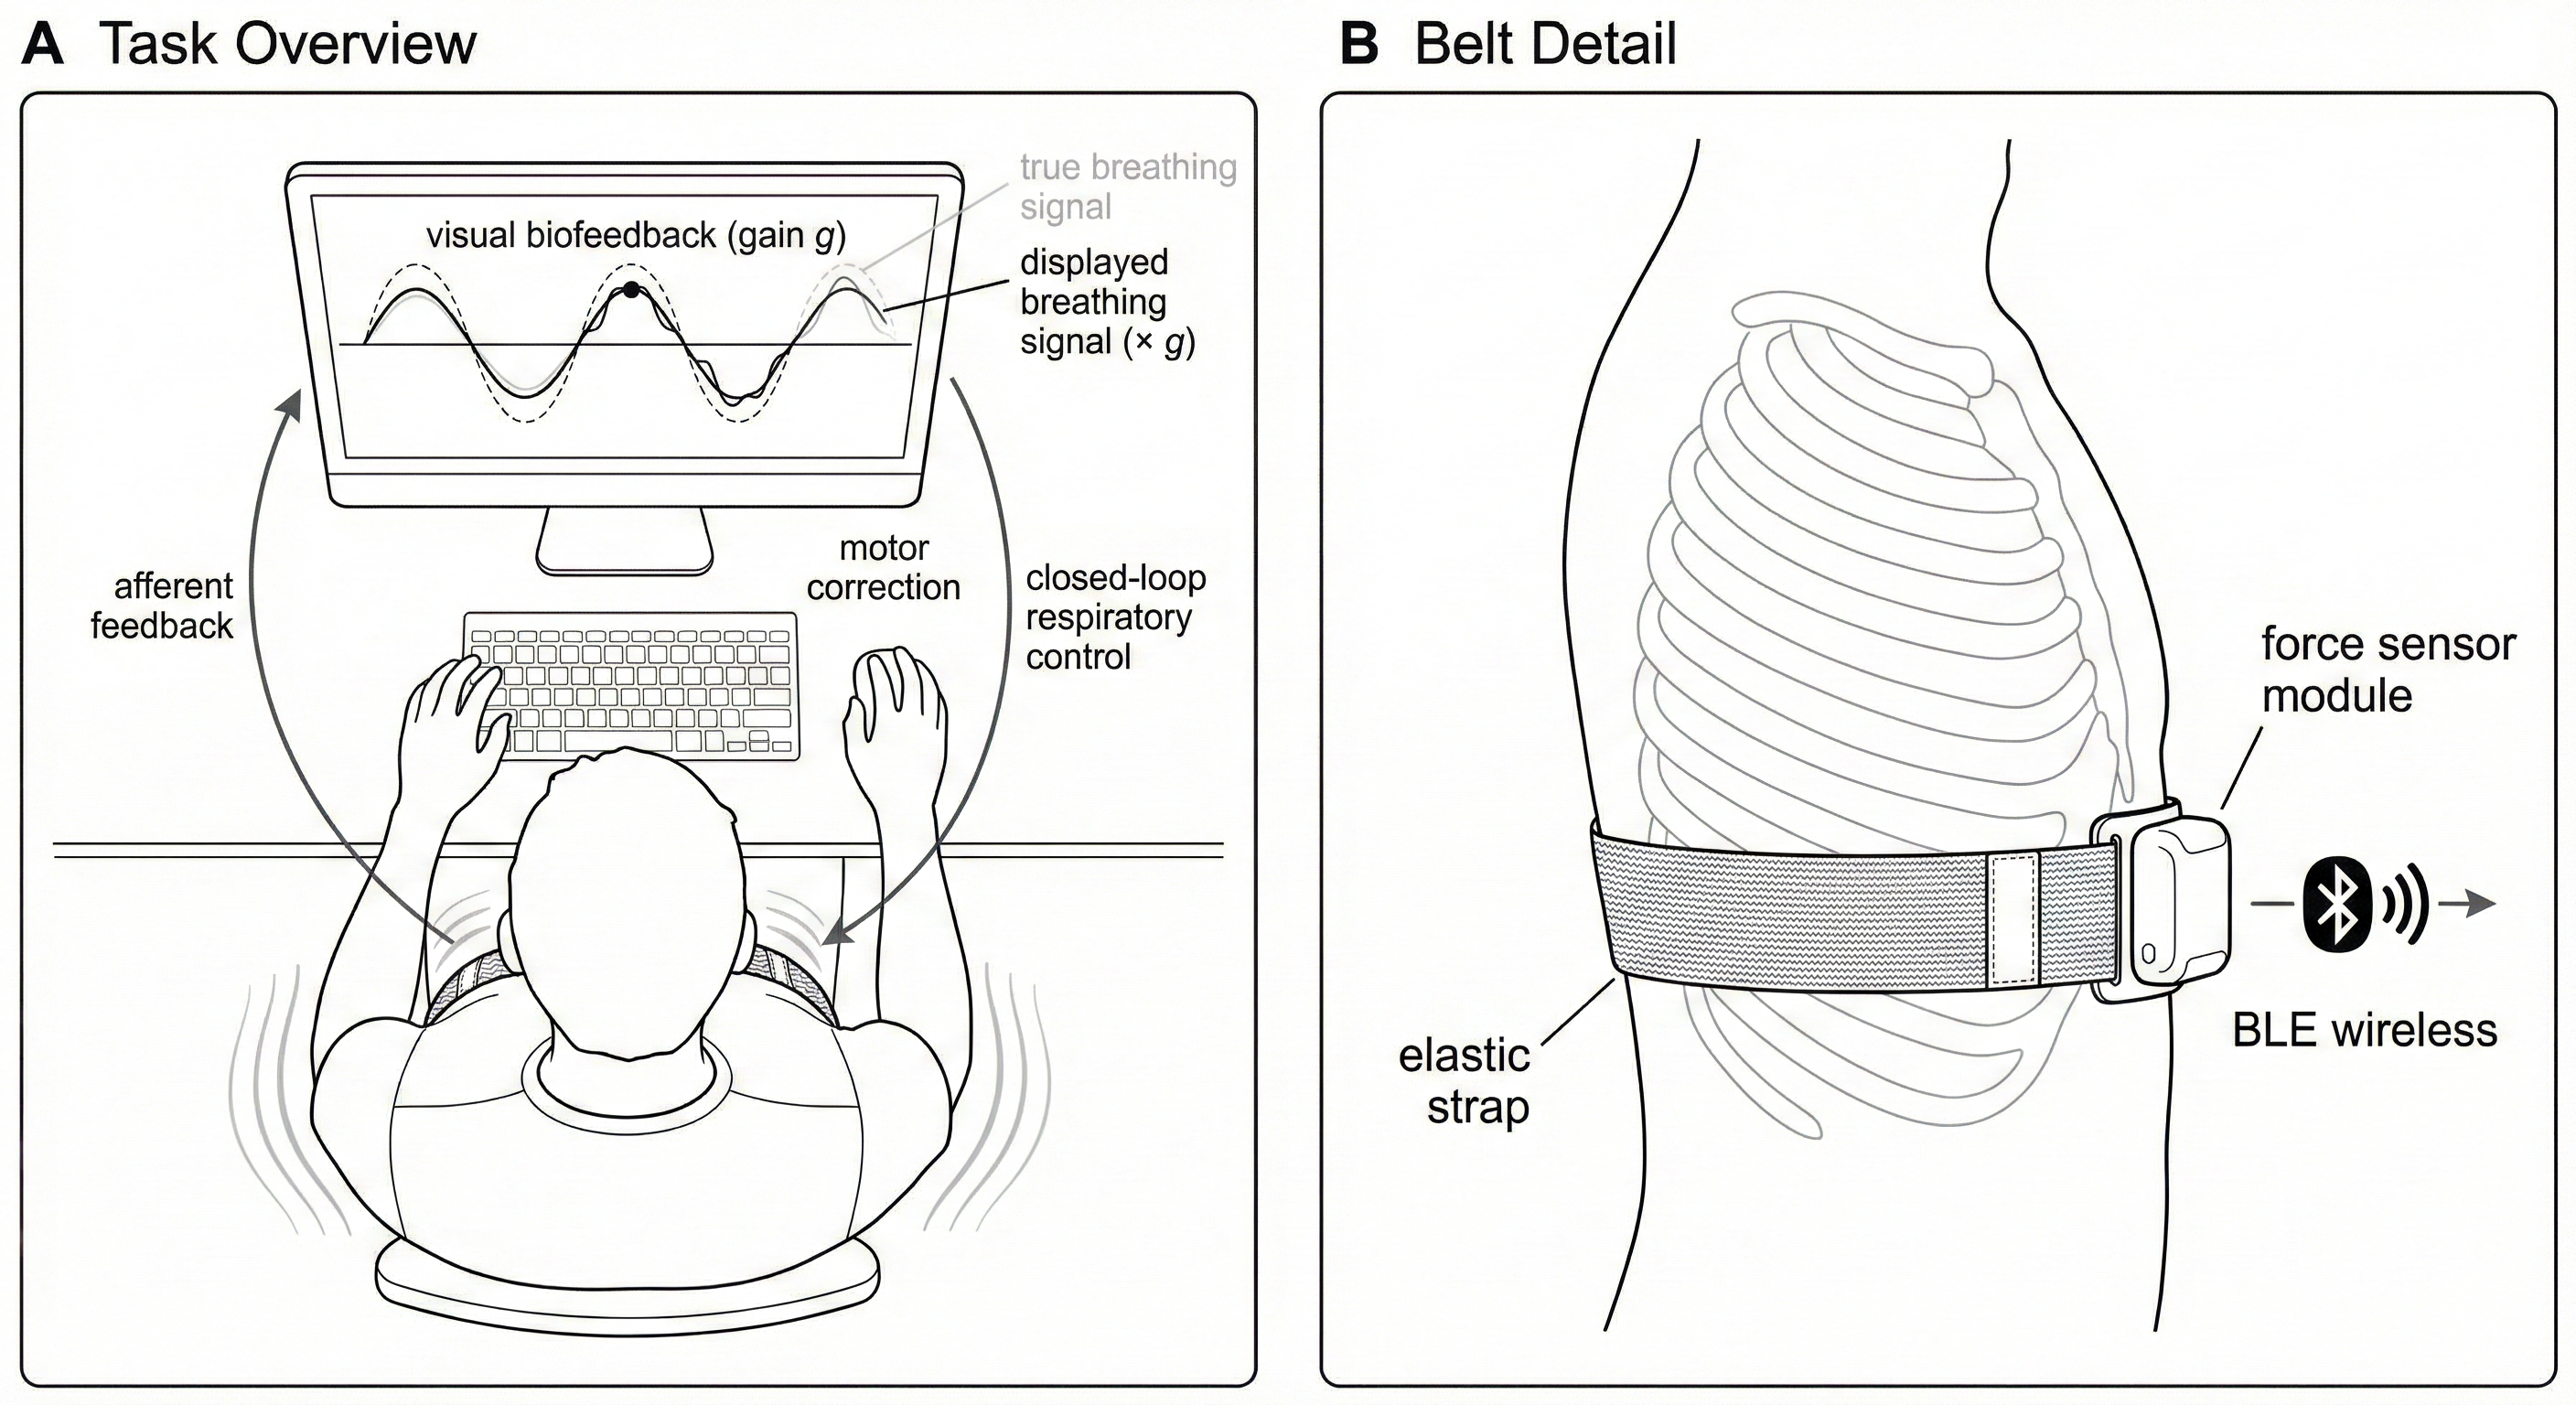
\includegraphics[width=\textwidth]{fig_task_schematic.png}
\caption{Schematic of the respiromotor tracking task. \textbf{(A)}~Task overview: the participant wears a respiration belt and views a monitor displaying their breathing trace in real time. A sinusoidal target guides the desired breathing pattern. Visual biofeedback can be veridically displayed or scaled by a gain factor $g$, creating a closed-loop sensorimotor control paradigm with afferent feedback and motor correction. \textbf{(B)}~Belt detail: the Vernier Go Direct Respiration Belt (GDX-RB) consists of an elastic strap with an embedded force sensor module that transmits data wirelessly via Bluetooth Low Energy (BLE).}
\label{fig:schematic}
\end{figure}

\subsection{Toolbox Architecture}

\textit{respyra} is implemented in Python 3.10 and integrates two primary components: the Vernier Go Direct Respiration Belt (GDX-RB; Vernier Software \& Technology) for real-time force-based respiratory measurement, and PsychoPy \parencite{peirce2019psychopy} for stimulus presentation and experiment control. The toolbox is organized into reusable core modules, configuration files, and experiment scripts, following a separation-of-concerns architecture (see Table~\ref{tab:modules}).

\begin{table}[ht]
\caption{Core Modules of the respyra Toolbox}
\label{tab:modules}
\begin{tabular}{lp{10cm}}
\toprule
Module & Description \\
\midrule
\texttt{breath\_belt} & Non-blocking interface to the Vernier GDX-RB. A background thread continuously reads force samples (10~Hz) into a thread-safe queue, allowing the main PsychoPy frame loop to drain samples without blocking. Supports BLE and USB connections. \\
\texttt{display} & PsychoPy window management and a \texttt{SignalTrace} class that renders a scrolling waveform by updating \texttt{ShapeStim} vertices each frame. \\
\texttt{target\_generator} & Generates sinusoidal breathing targets from composable frequency--cycle segment definitions. Supports multi-segment waveforms with phase-continuous boundaries. \\
\texttt{data\_logger} & Incremental CSV logging with per-row flush for crash resilience. \\
\texttt{events} & Keyboard input helpers wrapping PsychoPy's event module. \\
\bottomrule
\end{tabular}
\end{table}

The respiration belt measures chest expansion force in Newtons (0--50~N range) via a force sensor embedded in an elastic chest strap. The belt communicates with the host computer via Bluetooth Low Energy (BLE) or USB. To resolve a platform-specific conflict on Windows---where PsychoPy's graphics backend initializes COM in single-threaded apartment (STA) mode while the BLE scanner requires multi-threaded apartment (MTA) mode---the toolbox connects the belt \textit{before} importing PsychoPy modules.

Experimental conditions are defined using a \texttt{ConditionDef} dataclass specifying a name, a list of \texttt{SegmentDef} objects (each with a target frequency in Hz and an integer cycle count), and an optional \texttt{feedback\_gain} parameter. The use of integer cycle counts ensures phase continuity at segment boundaries, allowing seamless composition of multi-frequency waveforms.

\subsection{Visual Feedback and Perturbation}

The task display consists of two visual elements: a scrolling waveform trace showing the participant's real-time breathing signal, and a target dot that traverses a sinusoidal path at the prescribed target frequency. The dot's vertical position indicates the target force, and its color provides continuous error feedback using an HSV color mapping from green (low error) through yellow to red (high error), with a square-root transfer function for perceptual salience.

The visuomotor perturbation is implemented as a multiplicative gain applied exclusively to the visual trace display:
\begin{equation}
f_{\text{display}} = c + g \cdot (f_{\text{actual}} - c)
\label{eq:gain}
\end{equation}
where $f_{\text{actual}}$ is the raw belt force, $c$ is the participant's breathing center (from calibration), and $g$ is the feedback gain. When $g = 1.0$, the display is veridical. When $g > 1.0$, displayed deviations from center are amplified, requiring the participant to breathe with \textit{smaller} amplitude to match the visual target. Critically, the target dot position, tracking error computation, and dot color feedback all remain based on the unperturbed signal, isolating the perturbation to the sensory feedback channel.

\subsection{Calibration}

Prior to the experimental trials, participants complete a 15-second range calibration phase during which they take several comfortable deep breaths. The force data collected during this phase are used to establish the participant's achievable breathing range. To ensure robust calibration, the toolbox applies percentile-based outlier rejection (5th--95th percentile clipping), excluding extreme values caused by movement artifacts or sensor saturation. If force values approach the sensor limits ($\leq$~\SI{0}{\newton} or $\geq$~\SI{40}{\newton}), a warning dialog alerts the experimenter that the belt may be too tight. The clipped range is then scaled by a configurable factor (default 0.80) to set the target waveform amplitude, ensuring the sinusoidal target stays within the participant's comfortable range.

\subsection{Experimental Protocol}

Each session consists of a range calibration phase followed by a series of tracking trials. Each trial comprises three phases:

\begin{enumerate}
\item \textbf{Baseline} (10~s): The participant breathes naturally. Force data from this phase are used to compute a trial-specific breathing center via the midpoint of the observed range.
\item \textbf{Countdown} (3~s): A ``3\ldots2\ldots1'' countdown during which the target dot smoothly blends from the participant's current respiratory position into the target waveform trajectory, providing a gradual transition into tracking.
\item \textbf{Tracking} (30~s): The participant follows the sinusoidal target dot with their breathing. Force, target, and signed error are logged at every sample (\textasciitilde10~Hz). At the conclusion of each trial, mean absolute tracking error is displayed as performance feedback.
\end{enumerate}

Trial conditions are managed using PsychoPy's \texttt{TrialHandler}, supporting both sequential (alternating) and randomized presentation orders across configurable numbers of repetitions.

\subsection{Proof-of-Concept Data Collection}

To validate the toolbox, a single experienced participant (male, first author) completed one session consisting of six tracking trials alternating between two conditions: \textit{slow\_steady} (3 sinusoidal cycles at 0.1~Hz, veridical feedback; $g = 1.0$) and \textit{perturbed\_slow} (identical target waveform with visual gain perturbation; $g = 1.5$). Trial order was sequential (alternating), with three repetitions of each condition. The belt was worn around the lower ribcage and connected via BLE at 10~Hz sampling. The display was presented on a 1920$\times$1080 monitor at 57~cm viewing distance.

\subsection{Data Analysis}

Tracking performance was quantified using mean absolute error (MAE) and root mean square error (RMSE) between the target and actual force signals during the 30-second tracking phases. Statistics were computed both per-trial and per-condition. All analyses used the raw CSV output from the toolbox, processed with pandas and NumPy in Python.

\section{Results}

\subsection{Calibration}

The range calibration phase yielded a raw force range of 0.01--3.96~N. After percentile clipping (P5/P95), the effective range was 0.10--2.79~N, with a center of 1.45~N and scaled amplitude of 1.07~N. Baseline breathing centers were stable across trials ($M$ = \SI{1.15}{\newton}, range: 1.08--1.21~N), indicating consistent resting breathing position throughout the session.

\subsection{Tracking Performance}

The participant achieved accurate respiratory tracking across all six trials, with an overall MAE of \SI{0.174}{\newton} (RMSE = \SI{0.219}{\newton}). Table~\ref{tab:results} presents per-trial performance metrics.

\begin{table}[ht]
\caption{Per-Trial Tracking Performance}
\label{tab:results}
\begin{tabular}{ccS[table-format=1.0]S[table-format=1.3]S[table-format=1.3]c}
\toprule
Trial & Condition & {Gain} & {MAE (N)} & {RMSE (N)} & {$n$ samples} \\
\midrule
1 & slow\_steady    & 1.0 & 0.114 & 0.141 & 300 \\
2 & perturbed\_slow & 1.5 & 0.253 & 0.289 & 300 \\
3 & slow\_steady    & 1.0 & 0.108 & 0.143 & 301 \\
4 & perturbed\_slow & 1.5 & 0.249 & 0.288 & 300 \\
5 & slow\_steady    & 1.0 & 0.100 & 0.127 & 300 \\
6 & perturbed\_slow & 1.5 & 0.217 & 0.253 & 300 \\
\bottomrule
\end{tabular}
\end{table}

\subsection{Effect of Visuomotor Perturbation}

The gain perturbation condition produced consistently higher tracking errors than veridical feedback. Across the three veridical trials, the mean MAE was \SI{0.107}{\newton} ($SD$ = \SI{0.007}{\newton}). Across the three perturbed trials ($g = 1.5$), the mean MAE was \SI{0.240}{\newton} ($SD$ = \SI{0.020}{\newton}), representing a 2.2-fold increase in tracking error. The perturbation effect was present from the first perturbed trial and remained stable across repetitions, though a modest improvement was observed from the first (MAE = \SI{0.253}{\newton}) to the third perturbed trial (MAE = \SI{0.217}{\newton}), suggesting partial adaptation within the session. Veridical trials also showed a slight improvement across the session (Trial~1: 0.114, Trial~5: 0.100~N), consistent with general task familiarization. Figure~\ref{fig:summary} presents the full session summary.

\begin{figure}[ht]
\centering
\includegraphics[width=\textwidth]{fig_session_summary.png}
\caption{Six-panel session summary for the proof-of-concept participant. \textit{Top left}: Full session force trace (green) with target overlay (orange dashes) across all phases. \textit{Top right}: Signed tracking error over time for each trial. \textit{Middle left}: Per-trial mean absolute error; blue bars = slow\_steady (veridical), magenta bars = perturbed\_slow ($g = 1.5$). \textit{Middle right}: Error distribution by condition (box plots). \textit{Bottom left}: Baseline calibration stability (center $\pm$ amplitude) across trials. \textit{Bottom right}: Summary statistics.}
\label{fig:summary}
\end{figure}

\section{Discussion}

We presented \textit{respyra}, an open-source toolbox for studying respiratory motor control through real-time tracking with visuomotor perturbation. The proof-of-concept data demonstrate that the system produces stable, high-quality respiratory tracking data at 10~Hz and that participants can achieve precise control of their breathing to follow prescribed sinusoidal targets.

The visuomotor perturbation condition---in which the visual trace of breathing was amplified by a factor of 1.5 around the participant's center---reliably increased tracking error while remaining learnable. This finding parallels results from the visuomotor reaching literature, where cursor gain perturbations produce immediate performance costs followed by gradual adaptation \parencite{krakauer2019motor}. The observed improvement from the first to the third perturbed trial suggests that respiratory sensorimotor adaptation follows a similar trajectory, though systematic studies with larger samples are needed to characterize the time course and completeness of adaptation.

The design choice to apply the perturbation exclusively to the visual trace---while preserving veridical target positioning, error computation, and color feedback---creates a clean dissociation between the sensory feedback channel and the motor control reference signal. This mirrors the logic of cursor rotation paradigms in reaching studies, where the visual feedback is altered but the task goal (reach to the target) remains unchanged. Future work could explore whether respiratory adaptation to visual gain perturbation shows hallmarks of implicit sensorimotor recalibration (e.g., aftereffects when returning to veridical feedback) versus explicit strategic compensation.

The toolbox addresses several practical challenges in respiratory psychophysics. The percentile-based calibration with saturation detection provides robust target scaling even when individual data contain outlier breaths or sensor artifacts. The non-blocking belt interface ensures that respiratory sampling does not disrupt PsychoPy's frame-locked timing. The modular architecture---separating belt I/O, display rendering, target generation, and data logging into independent components---facilitates extension to new experimental designs.

Several limitations should be noted. First, the proof-of-concept data come from a single experienced participant (the developer), and performance may differ substantially in naive participants. Second, the current implementation uses a simple sinusoidal target; more complex waveforms (e.g., asymmetric inspiration/expiration ratios or naturalistic breathing patterns) may better capture the demands of real-world breathing regulation. Third, the 10~Hz sampling rate, while sufficient for tracking slow breathing patterns (\textasciitilde0.1~Hz), may limit the resolution of fine-grained error dynamics.

The respiratory motor control tracking paradigm opens several directions for future research. Within the interoceptive framework, the task could be combined with measures of respiratory interoceptive sensitivity \parencite{nikolova2022respiratory} to investigate whether perceptual sensitivity predicts motor control precision. The perturbation conditions could be extended to study sensorimotor adaptation dynamics---including savings, interference, and transfer---using the well-developed theoretical toolkit from the motor learning literature. Finally, the framework could support investigations of breathing-based interventions by quantifying how accurately individuals can implement prescribed breathing patterns (e.g., paced slow breathing at 0.1~Hz) and how this accuracy relates to downstream physiological and psychological outcomes \parencite{gholamrezaei2021psychophysiological, luo2025effect}.

\textit{respyra} is freely available at \url{https://github.com/embodied-computation-group/respyra} under an open-source license.

\printbibliography

\end{document}
